\section{Problem}
\subsection{Motivation}
\begin{frame}%\frametitle{Motivation}
    \begin{block}{Motivation}
    \begin{itemize} 
    	\item Fiber-To-The-Home (FTTH) services have a large penetration throughout the world, and provides high data rates to the final customers.
    	\item The number of applications and services on the internet has grown exponentially.
    	\item A smart augmentation of the physical network is mandatory.
    	\item Since the deployment of fiber optics is an important economical investment, the topological network design of \emph{FTTH} networks should be revisited.
	\end{itemize} 
    \end{block}
\end{frame}

\subsection{Objectives}
\begin{frame}
	\frametitle{}
    \begin{block}{Objectives}
	\begin{itemize} 
    	\item The goal is to interconnect distinguished nodes, called terminals, using large level of redundancy, and simultaneously, meeting large reliable constraints. 
		\item Find a minimum cost solution that achieves a reliability threshold, where both nodes and
links can fail with given probabilities.
	\item Understand the impact on the reliability of the solution networks, by increasing or decreasing the basic reliability of both nodes and links.
	\item Understand the cost-reliability trade-off, and how the reliability is naturally increased adding levels of redundancy between distinguished terminals.
	\end{itemize} 
    \end{block}
\end{frame}

\subsection{Definition}
\begin{frame}\frametitle{Generalized Steiner Problem with Node-Connectivity Constraints and
Hostile Reliability (GSPNCHR)}
    \begin{definition}[GSPNCHR]
Consider a simple undirected graph $G=(V,E)$, terminal-set $T \subseteq V$, link-costs $\{c_{i,j}\}_{(i,j) \in E}$ and connectivity requirements $R=\{r_{i,j}\}_{i,j \in T}$. Further, we assume that both links and non-terminal (Steiner) nodes fail with respective probabilities $P_E=\{p_e\}_{e\in E}$ and $P_{V-T}=\{p_v\}_{v\in V-T}$. Given a reliability threshold $p_{min}$, the goal is to build a minimum-cost topology $G_S \subseteq G$ meeting both the connectivity requirements $R$ and the reliability threshold: $R_{K}(G_S) \geq p_{min}$, being $K=T$ the terminal-set.
\end{definition}
\end{frame}

\subsection{Combinatorial Optimization Problem}
\begin{frame}\frametitle{GSPNCHR}
\begin{align}
\min &\sum_{(i,j)\in E} c_{i,j}x_{i,j} \notag \\
s.t. x_{ij}&\geq y_{(i,j)}^{u,v}+y_{(j,i)}^{u,v} \forall (i,j)\in E,
\forall u,v\in T, u \neq v \\
\sum_{(u,i)\in E}y_{(u,i)}^{u,v} &\geq r_{u,v} \, \, \forall \, u,v\in T, \, u\neq v \\
\sum_{(j,v)\in E}y_{(j,v)}^{u,v} &\geq r_{u,v} \, \, \forall \, u,v\in T, \, u\neq v \\
\sum_{(i,p)\in I(p)}y_{(i,p)}^{u,v}  - \sum_{(p,j)\in I(p)}y_{(p,j)}^{u,v}&\geq 0, \, \forall p\in V-\{u,v\}, \, \forall u,v\in T, \, u \neq v \notag \\
\end{align}
\end{frame}

\subsection{Combinatorial Optimization Problem}
\begin{frame}\frametitle{GSPNCHR}
\begin{align}
\sum_{(s,i)\in E} x_{s,i} &\leq M \hat{x}_{s}, \, \forall s\in V-T \\
R_{K}(G_S(\{x_{ij}\})) &\geq p_{min} \\
x_{(i,j)} &\in \{0,1\} \, \forall (i,j)\in E \\
\hat{x}_{i} &\in \{0,1\} \, \forall i \in V-T  \\
 y_{(i,j)}^{u,v} &\in \{0,1\} \, \forall (i,j)\in E, \, \forall u,v \in T, \, u \neq v
\end{align}
\end{frame}

\section{Solution}
\subsection{Methodology}
\begin{frame}\frametitle{GRASP/VND}
\begin{block}{}
\begin{small}
\begin{itemize}
 \item GRASP and VND are well known metaheuristics that have been successfully used to solve many hard combinatorial optimization problems
 \item GRASP is a powerful multi-start process which operates in two phases. A feasible solution is built in a rst phase, whose neighborhood is then explored in the Local Search Phase. 
 \item VND explores several neighborhood structures in a deterministic order. Its success is based on the simple fact that different neighborhood structures do not usually have the same local minimum.
\end{itemize} 
\end{small}
\end{block}
\end{frame}

\subsection{General Scheme}
\begin{frame}\frametitle{}
    \begin{block}{Network Design}
\begin{algorithm}[H]
\floatname{algorithm}{Alg}
\caption{$sol = NetworkDesign(G_B,iter,k,p_{min},P_E,P_{V-T},simiter)$}
\begin{algorithmic}[1]
\begin{small}    
\STATE $i \leftarrow 0; \, P \leftarrow \emptyset; \, sol \leftarrow \emptyset$
\WHILE {$i < iter$}
\STATE $\overline{g} \leftarrow Construction(G_B,P,k)$
\STATE $g_{sol} \leftarrow VND(\overline{g},P)$
\STATE $reliability \leftarrow RVR(g_{sol},P_E,P_{V-T},simiter)$
\IF{$reliability > p_{min}$}
\STATE $sol \leftarrow sol \cup \{g_{sol}\}$
\ENDIF
\ENDWHILE
\RETURN $sol$
\end{small}
\end{algorithmic}
\end{algorithm}
    \end{block}
\end{frame}

\subsection{Construction Phase}
\begin{frame}\frametitle{}
    \begin{block}{}
\begin{algorithm}[H]
\floatname{algorithm}{Alg}
\caption{$(sol,P) = Construction(G_B,C,R,k)$}
\begin{algorithmic}[1]
\begin{scriptsize}
\STATE $g_{sol} \leftarrow (S_D^{(I)},\emptyset)$; $m_{i,j}\leftarrow r_{i,j}$; $P_{i,j}\leftarrow \emptyset, \forall i,j \in S_{D}^{(I)}$; $A_{i,j}\leftarrow 0, \forall i,j \in S_{D}^{(I)}$
\WHILE {$\exists \, m_{i,j}>0: A_{i,j}<MAXATTEMPTS$}
\STATE $(i,j) \leftarrow ChooseRandom(S_{D}^{(I)}: m_{i,j}>0)$
\STATE $\overline{G} \leftarrow G_B \setminus P_{i,j}$
\FORALL {$(u,v)\in E(\overline{G})$}
\STATE $\overline{c}_{u,v} \leftarrow c_{u,v} \times 1_{\{(u,v) \notin g_{sol}\}}$
\ENDFOR
\STATE $L_p \leftarrow KSP(k,i,j,\overline{G},\overline{C})$
\IF{$L_p=\emptyset$}
\STATE $A_{i,j} \leftarrow A_{i,j}+1$; $P_{i,j} \leftarrow \emptyset$; $m_{i,j}\leftarrow r_{i,j}$ 
\ELSE 
\STATE $p \leftarrow SelectRandom(L_p)$; $g_{sol} \leftarrow g_{sol} \cup \{p\}$
\STATE $P_{i,j} \leftarrow P_{i,j} \cup \{p\}$; $m_{i,j} \leftarrow m_{i,j}-1$
\STATE $(P,M) \leftarrow GeneralUpdateMatrix(g_{sol},P,M,p,i,j)$
\ENDIF
\ENDWHILE
\RETURN $(g_{sol},P)$
\end{scriptsize}    
\end{algorithmic}
\end{algorithm}
\end{block}
\end{frame}

\subsection{Local Search Phase}
\begin{frame}\frametitle{}
\begin{block}{VND}
\begin{small}
The goal is to combine a rich diversity of neighborhoods in order to obtain an output that is locally optimum solution for every feasible neighborhood. Here, we consider three neighborhood structures to build a VND.
\begin{enumerate}
 \item SwapKeyPathLocalSearch
 \item KeyPathLocalSearch
 \item KeyTreeLocalSearch
\end{enumerate} 
\end{small}
\end{block}
\end{frame}

\subsection{SwapKeyPathLocalSearch}
\begin{frame}\frametitle{}
%\begin{small}
%\begin{definition}[Estructura de Vecindad para Swap Key-Paths]
%Dado un key-path $p \subseteq g_{sol}$, una solución vecina para $g_{sol}$ es 
%$\hat{g}_{sol} = \{ g_{sol}\setminus p \}\cup \{m\}$, 
%siendo $m$ el conjunto de nodos y enlaces que serán añadidos preservando la factibilidad de ${\hat{g}}%_{sol}$.  
%\end{definition}
%\end{small}
\begin{block}{}
\begin{algorithm}[H]
\floatname{algorithm}{Alg}
\caption{$g_{sol} = SwapKeyPathLocalSearch(G_B,C,g_{sol},P)$}
\begin{algorithmic}[1]
\begin{scriptsize}
\STATE $improve \leftarrow TRUE$
\WHILE {$improve$}
\STATE $improve \leftarrow FALSE$
\STATE $K(g_{sol}) \leftarrow \{p_1,\ldots,p_h\}$ /* Key-path decomposition of $g_{sol}$ */
\WHILE{\textbf{not} $improve$ \textbf{and} $\exists$ \textbf{key-paths not analyzed}}
\STATE $p \leftarrow(K(g_{sol}))$ /* Path not analyzed yet */
\STATE $(g_{sol},improve) \leftarrow FindSubstituteKeyPath(g_{sol},p,P)$
\ENDWHILE
\ENDWHILE
\RETURN $g_{sol}$
\end{scriptsize}
\end{algorithmic}
\end{algorithm}
\end{block}
\end{frame}

\subsection{KeyPathLocalSearch}
\begin{frame}\frametitle{}
%\begin{definition}[Estructura de Vecindad para Key-Paths]
%\begin{tiny}
%Dado un key-path $p \in g_{sol}$, una solución vecina es 
%${\hat{g}}_{sol} = \{g_{sol} \setminus p \} \cup \{\hat{p}\}$, 
%donde $\hat{p}$ es otro camino que conecta los extremos desde $p$.  
%La vecindad de key-paths desde $g_{sol}$ esta compuesta por la operación previa 
%a los posibles miembros pertenecientes a $K_{g_{sol}}$. 
%\end{tiny}
%\end{definition}
\begin{block}{}
\begin{algorithm}[H]
\floatname{algorithm}{Alg}
\caption{$g_{sol} = KeyPathLocalSearch(G_B,C,g_{sol})$}
\begin{algorithmic}[1]
\begin{tiny}
\STATE $improve \leftarrow TRUE$
\WHILE {$improve$}
\STATE $improve \leftarrow FALSE$
\STATE $K(g_{sol}) \leftarrow \{p_1,\ldots,p_h\}$ /* Key-path decomposition of $g_{sol}$ */
%\COMMENT{Key-path decomposition of $g_{sol}$}
\WHILE{\textbf{not} $improve$ \textbf{and} $\exists$ \textbf{key-paths not analyzed}}
\STATE $p \leftarrow(K(g_{sol}))$ /* Path not analyzed yet, with extremes $u$ and $v$ */
\STATE $\hat{\mu} \leftarrow <NODES(p) \cup S_D\setminus NODES(g_{sol}) > $ /* Induced subgraph $\hat{\mu}$ */
\STATE $\hat{p} \leftarrow Dijkstra(u,v,\hat{\mu})$
\IF{$COST(\hat{p}) < COST(p)$}
\STATE $g_{sol} \leftarrow \{ g_{sol}\setminus p \} \cup \{\hat{p}\}$
\STATE $improve \leftarrow TRUE$
\ENDIF
\ENDWHILE
\ENDWHILE
\RETURN $g_{sol}$
\end{tiny}
\end{algorithmic}
\end{algorithm}
\end{block}
\end{frame}

\subsection{KeyTreeLocalSearch}
\begin{frame}\frametitle{}
%\begin{definition}[Estructura de Vecindad para Key-Tree]
%\begin{small}
%Se considera el key-tree $T_v \in g_{sol}$ con raíz key-node $v$.  
%Un vecino de $g_{sol}$ es $\hat{g}_{sol} = \{ g_{sol}\setminus T_v \} \cup \{T\}$, siendo 
%$T$ otro árbol que reemplaza a $T_v$ con hojas identicas. 
%\end{small}
%\end{definition}
\begin{block}{}
\begin{algorithm}[H]
\floatname{algorithm}{Alg}
\caption{$g_{sol} = KeyTreeLocalSearch(G_B,C,g_{sol})$}
\begin{algorithmic}[1]
\begin{scriptsize}
\STATE $improve \leftarrow TRUE$
\WHILE {$improve$}
\STATE $improve \leftarrow FALSE$
\STATE $ X \leftarrow KeyNodes(g_{sol})$ /* Key-nodes from $g_{sol}$ */
\STATE $\overline{S} \leftarrow S_D \setminus NODES(g_{sol})$
\WHILE{\textbf{not} $improve$ \textbf{and} $\exists$ \textbf{key-nodes not analyzed}}
\STATE $v \leftarrow X$ /* Key-node not analyzed yet */
\STATE $[g_{sol},improve] \leftarrow GeneralRecConnect(G_B,C,g_{sol},v,\overline{S})$
\ENDWHILE
\ENDWHILE
\RETURN $g_{sol}$
\end{scriptsize}
\end{algorithmic}
\end{algorithm}
\end{block}
\end{frame}

\subsection{Confiabilidad}
\begin{frame}\frametitle{}
\begin{block}{RVR}
\begin{scriptsize}
\begin{itemize}
 \item Recursive Variance Reduction Method.
 \item Objective to reduce the original network into several smaller networks recursively.
 \item Construct an unbiased estimator of reliability, with less variance than the raw Monte Carlo.
 %Sistema Binario Estocastico Monoto. 
\end{itemize} 
\end{scriptsize}
\end{block}
\begin{block}{}
\begin{algorithm}[H]
\floatname{algorithm}{Alg}
\caption{$RVR(G,K,p_v,p_e)$}
\begin{algorithmic}[1]
\begin{tiny}
\STATE \textbf{If} $terminals$=1, \textbf{return} $0$
\STATE \textbf{Elseif} $\phi(G,K)=1$, \textbf{return} 1.
\STATE \textbf{Else} 
\STATE $D := GetKExtendedCut(G)$
\STATE $Q_{D} := AllFailedProb(D)$
\STATE $index := GetRandomItem(D)$
\STATE $c := D[index]$
\STATE $remove(G,D, index - 1)$
\STATE $add(G, c)$
\STATE $return \, \, Q_{D} + (1 - Q_{D})\times RVR(G)$
\STATE \textbf{EndIf}
\end{tiny}
\end{algorithmic}
\end{algorithm}
\end{block}
\end{frame}

\section{Numerical Results}
\subsection{Numerical Results}
\begin{frame}\frametitle{}
\begin{block}{Test Set}
\begin{small}
\begin{itemize}
 \item An extensive computational study was conducted using the $NetworkDesign$ algorithm.
 \item We adapt known instances of the  $TSPLIB$  library adapting them to our problem adding probabilities of failure in nodes and edges and the connectivity requirements between nodes.
 \item There are no benchmark cases for our specific problem.
 \item Reliability threshold $p_{min}=0.8$.
 \item Node and edge reliabilities $p_v=0.99$ y $p_e=0.95$ respectively.
 \item Number of iterations in $NetworkDesign$ for each instance $iter=100$, and number of replications for the $RVR$ $10^4$ simulation method.
 \item We want to understand the sensitivity of the solution to disturbances in elementary reliabilities. Therefore, different values were used for the elementary reliabilities for both the Steiner nodes and links $p_{v},p_{e} \in \{0.99, 0.97,0.95\}$.
\end{itemize} 
\end{small}
\end{block}
\end{frame}

\subsection{Numerical Results II}
\begin{frame}\frametitle{}
\begin{table}
\begin{scriptsize}
\caption{Test Set}
\end{scriptsize}
\centering
\scalebox{0.7}{
\begin{tabular}{|c|c|c|c|c|c|c|c|} % centered columns 
\hline	$Problem$   &	\% $T$ & \%$Rel$& \% $Req$ & $Iter\_ND$ & $Iter\_RVR$ & \# \\
\hline	att48	&	20-35-50	&	99-95	&	100-0-0	&	100-100-100	&	$10^4$	&	3	\\
\hline	berlin52	&	20-35-50	&	99-95	&	100-0-0	&	100-100-100	&	$10^4$	&	3	\\
\hline	brazil58	&	20-35-50	&	99-95	&	100-0-0	&	100-100-100	&	$10^4$	&	3	\\
\hline	ch150	&	20-35-50	&	99-95	&	100-0-0	&	100-100-100	&	$10^4$	&	3	\\
\hline	d198	&	20-35-50	&	99-95	&	100-0-0	&	20-20-20	&	NA	&	3	\\
\hline	eil51	&	20-35-50	&	99-95	&	100-0-0	&	100-100-100	&	$10^4$	&	3	\\
%\hline	gr137	&	20-35-50	&	99-95	&	100-0-0	&	100-20-20	&	NA	&	3	\\
\hline	gr202	&	20-35-50	&	99-95	&	100-0-0	&	100-100-100	&	$10^4$	&	3	\\
\hline	kroA100	&	20-35-50	&	99-95	&	100-0-0	&	100-100-100	&	NA	&	3	\\
%\hline	kroA150	&	20-35-50	&	99-95	&	100-0-0	&	100-20-20	&	NA	&	3	\\
\hline	kroB100	&	20-35-50	&	99-95	&	100-0-0	&	100-100-100	&	NA	&	3	\\
\hline	kroB150	&	20-35-50	&	99-95	&	100-0-0	&	100-20-20	&	NA	&	3	\\
\hline	kroB200	&	20-35-50	&	99-95	&	100-0-0	&	20-20-20	&	NA	&	3	\\
\hline	lin105	&	20-35-50	&	99-95	&	100-0-0	&	100-100-100	&	NA	&	3	\\
\hline	pr152	&	20-35-50	&	99-95	&	100-0-0	&	20-20-20	&	NA	&	3	\\
%\hline	rat195	&	20-35-50	&	99-95	&	100-0-0	&	20-20-20	&	NA	&	3	\\
%\hline	st70	&	20-35-50	&	99-95	&	100-0-0	&	100-100-100	&	$10^4$	&	3	\\
\hline	tsp225	&	20-35-50	&	99-95	&	100-0-0	&	50-50-50	&	$10^4$	&	3	\\
%\hline	u159	&	20-35-50	&	99-95	&	100-0-0	&	20-20-20	&	NA	&	3	\\
%\hline	rd100	&	20-35-50	&	99-95	&	100-0-0	&	100-100-100	&	NA	&	3	\\
\hline	rd400	&	20-35-50	&	99-95	&	100-0-0	&	50-50-50	&	$10^4$	&	3	\\
\hline	berlin52(E)	&	20	&	99-90	&	65-25-10	&	100	&	$10^4$	&	1	\\
%\hline	eil51(E)	&	20	&	99-90	&	65-25-10	&	100	&	$10^4$	&	1	\\
\hline	att48(E)	&	35	&	99-90	&	65-25-10	&	100	&	$10^4$	&	1	\\
%\hline	st70(E)	&	35	&	99-90	&	65-25-10	&	100	&	$10^4$	&	1	\\
\hline	brazil58(E)	&	50	&	99-90	&	65-25-10	&	100	&	$10^4$	&	1	\\
%\hline	eil51(E)	&	50	&	99-90	&	65-25-10	&	100	&	$10^4$	&	1	\\
%\hline	kroB100(E)	&	20	&	99-90	&	65-25-10	&	100	&	$10^4$	&	1	\\
%\hline	lin105(E)	&	20	&	99-90	&	65-25-10	&	100	&	NA	&	1	\\
%\hline	kroA100(E)	&	35	&	99-90	&	65-25-10	&	20	&	$10^4$	&	1	\\
\hline	rd100(E)	&	35	&	99-90	&	65-25-10	&	20	&	NA	&	1	\\
\hline
\end{tabular}}
\end{table}
\end{frame}

\subsection{Numerical Results III}
\begin{frame}\frametitle{}
\begin{table}
\begin{scriptsize}
\caption{GRASP/VND Effectiveness}
\end{scriptsize}
\centering
\scalebox{0.7}{
\begin{tabular}{|c|c|c|c|c|c|c|} % centered columns 
\hline	$Problem$   &	\% $T$ & \%$IC$& \% $IVND$ & $CPU(s)$ & $\overline{R}$ & $\overline{Var}$ \\
\hline	att48	&	20	&	99.27	&	34.61	&	11.466	&	0.967	&	7.608E-07	\\
\hline	att48	&	35	&	98.6	&	36.83	&	29.769	&	0.943	&	3.448E-06	\\
\hline	att48	&	50	&	98.22	&	37.1	&	65.904	&	0.927	&	5.322E-06	\\
\hline	berlin52	&	20	&	98.98	&	30.55	&	30.605	&	0.937	&	3.294E-06	\\
\hline	berlin52	&	35	&	99.06	&	33.93	&	33.433	&	0.938	&	3.19E-06	\\
\hline	berlin52	&	50	&	98.02	&	33.48	&	106.945	&	0.907	&	6.487E-06	\\
\hline	brazil58	&	20	&	98.92	&	31.96	&	62.377	&	0.885	&	6.722E-06	\\
\hline	brazil58	&	35	&	99.25	&	39.45	&	68.891	&	0.86	&	8.347E-06	\\
\hline	brazil58	&	50	&	98.75	&	35.26	&	103.553	&	0.91	&	7.093E-06	\\
\hline	ch150	&	20	&	99.76	&	37.51	&	222.552	&	0.8559	&	1.029E-05	\\
\hline	ch150	&	35	&	99.72	&	36.65	&	546.652	&	0.8803	&	9.033E-05	\\
\hline	gr202	&	20	&	99.89	&	32.43	&	100.162	&	0.8231	&	1.224E-05	\\
\hline	gr202	&	35	&	99.75	&	34.56	&	200.698	&	0.8414	&	1.11E-05	\\
\hline	gr202	&	50	&	99.74	&	33.36	&	600.629	&	0.8303	&	1.279E-05	\\
\hline	rd400	&	20	&	99.94	&	35.84	&	88.214	&	0.8094	&	14.22E-05	\\
\hline	rd400	&	35	&	99.94	&	33.54	&	504.103	&	0.8537	&	11.89E-05	\\
\hline	rd400	&	50	&	99.93	&	33.16	&	980.701	&	0.8643	&	11.51E-05	\\
\hline Average     & 35    &   99.28   &  34.72   &    220.980 &  0.884 & 3.28E-05 \\
\hline
\end{tabular}}
\end{table}
\end{frame}

\subsection{Numerical Results IV}
\begin{frame}\frametitle{}
\begin{block}{Brazil58}
\begin{scriptsize}
20\% terminals nodes, elemental reliability of Steiner nodes 99\%, link reliability 95\% and 100\% 2 node-disjoint paths. Red terminal nodes do not fail, orange and gray Steiner nodes.
\end{scriptsize}
\begin{center}
   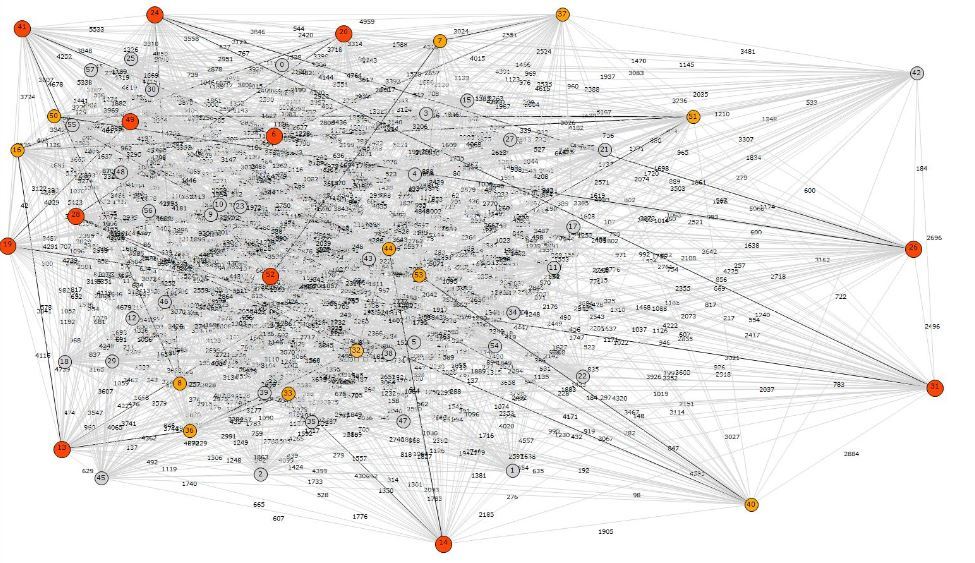
\includegraphics[scale=0.35]{figuras/1}
\end{center}
\end{block}
\end{frame}

\subsection{Numerical Results V}
\begin{frame}\frametitle{}
\begin{block}{Brazil58 NetworkDesign Output}
\begin{scriptsize}
Result cost 25106 (32\% improvement over construction) and reliability 92\%. 
\end{scriptsize}
\begin{center}
   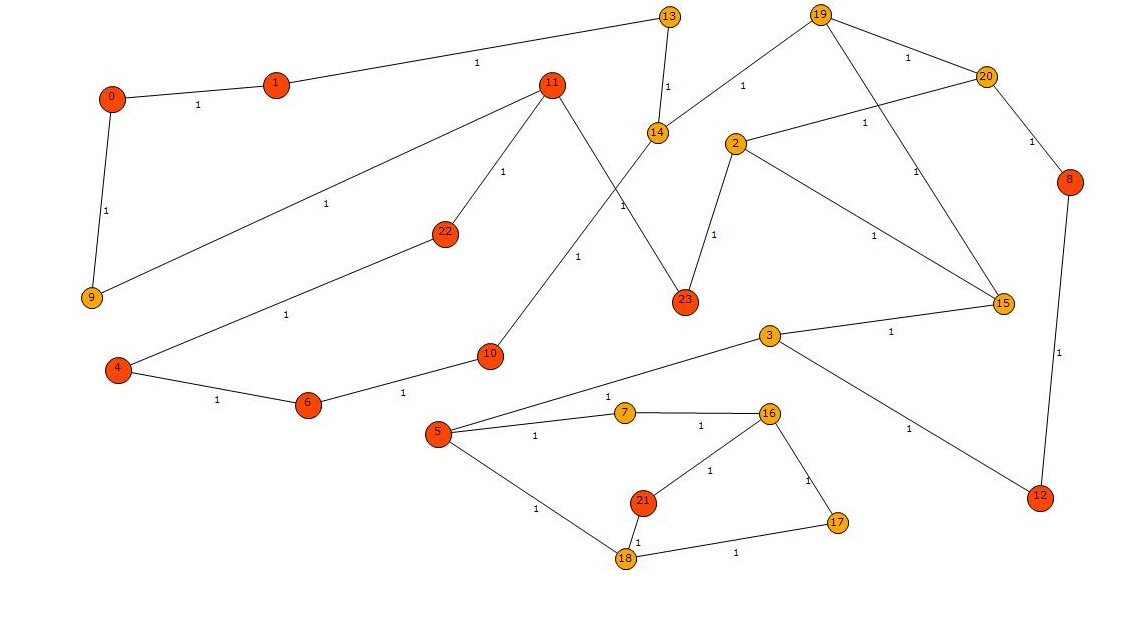
\includegraphics[scale=0.35]{figuras/2}
\end{center}
\end{block}
\end{frame}

\section{Conclusions}
\subsection{Conclusions}
\begin{frame} \frametitle{Contributions of this work}
\begin{block} {}
   	\begin{itemize} 
   	\begin{scriptsize}
	\item We study the topological design of high reliability networks.
	\item Our goal is to combine purely deterministic aspects such as connectivity with probabilistic models derived from network reliability.
	\item The Generalized Steiner Problem with Node-Connectivity Constraints and Hostile Reliability (GSPNCHR) is introduced.
	\item We formally prove that GSPNCHR belongs to the NP-Hard class.
	\item As a consequence, a GRASP / VND methodology is proposed.
	\end{scriptsize}   	     	
 	\end{itemize} 	
 \end{block}
\end{frame}

\subsection{Conclusions II}
\begin{frame} \frametitle{Conclusions}
\begin{block} {}
   	\begin{itemize} 
   	\begin{scriptsize}
	\item Since the reliability assessment for the hostile model also belongs to the NP-Hard class, we adopt an excellent point reliability estimate, known as Recursive Variance Reduction (RVR). This method is unbiased, accurate, and has small variance, as the results show.
	\item The improvement provided by the VNS phase after Greedy Construction ranges from 25.25% to 39.84%.
	\item Average reliability for all networks varies between 82.31% and 99.87%.
	\item Our results highlight that the model is robust under non-terminal node-failures, rather than link-failures.
	\end{scriptsize}   	     	
 	\end{itemize} 	
 \end{block}
\end{frame}

\subsection{Thanks}
\begin{frame} \frametitle{End}
\begin{huge}
\begin{center}Thanks for your attention.\end{center}
\end{huge}
\end{frame}

\section{Anexos}
\subsection{Anexo}
\begin{frame}\frametitle{}
\begin{block}{Berlin52}
\begin{scriptsize}
20\% de nodos terminales, confiabilidad elemental de nodos de Steiner 99\%, confiabilidad de enlaces 95\% y 100\% 2 caminos nodo-disjuntos.  Nodos terminales rojos no fallan, nodos de Steiner naranjas y grises.
\end{scriptsize}
\begin{center}
   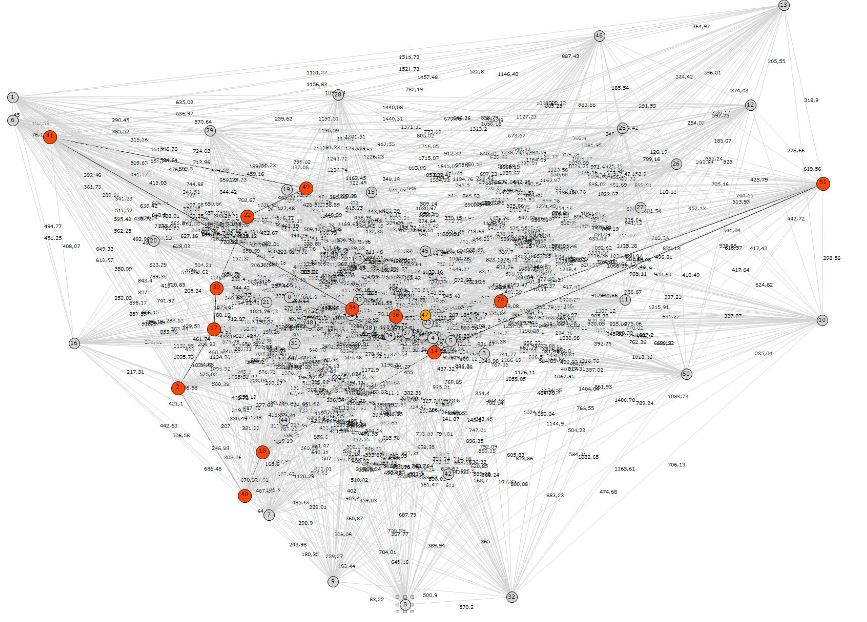
\includegraphics[scale=0.35]{figuras/3}
\end{center}
\end{block}
\end{frame}

\subsection{Anexo II}
\begin{frame}\frametitle{}
\begin{block}{Berlin52 Salida NetworkDesign}
\begin{scriptsize}
Costo resultado 4534 (31\% de mejora con respecto a la de construcción) y confiabilidad 84\%.
\end{scriptsize}
\begin{center}
   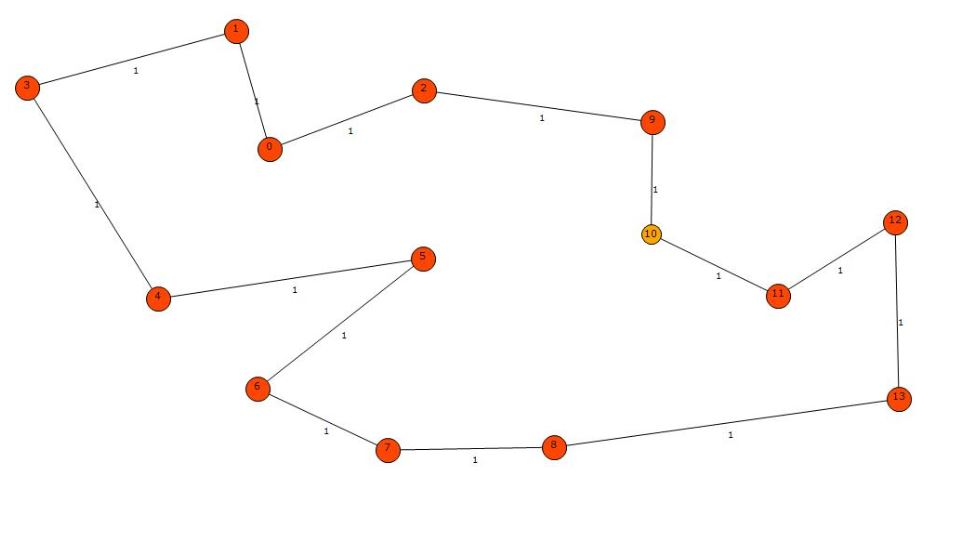
\includegraphics[scale=0.35]{figuras/4}
\end{center}
\end{block}
\end{frame}

\subsection{Definiciones}
\begin{frame}\frametitle{}
\begin{definition}[key-node]
Un key-node $v$ en una solución factible $v \in g_{sol}$ es un nodo de Steiner (no terminal) con grado mayor o igual a tres.
\end{definition}
\begin{definition}[key-path]
Un key-path $p$ en una solución factible $p \subseteq g_{sol}$ es un camino elemental 
donde todos los nodos intermedios no son terminales con grado dos en $g_{sol}$, 
y los nodos extremos son terminales o key-nodes.
\end{definition}
\begin{definition}[key-tree]
Sea $v \in g_{sol}$ un key-node perteneciente a una solución factible $g_{sol}$. 
El key-tree asociado a $v$, denotado como $T_v$, es un árbol compuesto por todos los 
key-paths que se encuentran en un punto común (i.e., el key-node $v$).
\end{definition}
\end{frame}

\subsection{Numerical Results IV}
\begin{frame} \frametitle{Preguntas Claves}
\begin{tiny}
\begin{block} {1}
 	 \begin{itemize}
 	 	\item ¿Cuántas redes factibles superan el umbral de confiabilidad, dado el modelo probabilístico completo $(p_{min}:0.98,P_E:0.99,P_{V-T}:0.99)$?
 	 	\item La cantidad de soluciones que cumplen con el umbral de confiabilidad es alta. Alcanza el 100\% en la mayoría de los casos.
 	 \end{itemize}  
 \end{block} 	   
 \begin{block} {2}
 	 \begin{itemize}
 	 	\item ¿Cuál es la sensibilidad del modelo con respecto a las confiabilidades elementales? ¿Es mejor aumentar la confiabilidad elemental de los enlaces, o la confiabilidad de los nodos Steiner, para cumplir con un umbral de confiabilidad exigente?
 	 	\item El modelo es más sensible a fallas de enlaces que a fallas de nodos. Un aumento en la confiabilidad de los enlaces tiene un mayor impacto que un aumento correspondiente en la confiabilidad de los nodos.
 	 \end{itemize}  
 \end{block} 	
  \begin{block} {3}
 	 \begin{itemize}
 	 	\item ¿Cuántas redes sobreviven en promedio, para cualquier modelo probabilístico dado? Comprender la sensibilidad del modelo con respecto a los requisitos de conectividad $r_{i,j} \in \{2,3,4\}$?
 	 	\item Podemos apreciar que un aumento en los requisitos de conectividad de la red implica necesariamente un aumento correspondiente en el porcentaje de redes que cumplen con el umbral de confiabilidad, y viceversa.
 	 \end{itemize}  
 \end{block} 	
 \end{tiny}
\end{frame}

\subsection{Resultados V}
\begin{frame}\frametitle{}
\begin{table}
\begin{scriptsize}
\caption{Soluciones factibles con $R \geq 0.98$,  
$p_v=0.99$ fijo y confiabilidad de enlaces variable.}
\end{scriptsize}
\centering  % used for centering table
\scalebox{0.7}{
\begin{tabular}{|c|c|c|c|c|} % centered columns 
\hline	Instance  &	$p_e=0.99$ & 	$p_e=0.97$ & 	$p_e=0.95$\\
\hline	att48 T20	&	100	&	90	&	12	\\
\hline	att48 T35	&	100	&	53	&	0	\\
\hline	att48 T50	&	100	&	20	&	0	\\
\hline	berlin52 T20	&	100	&	41	&	0	\\
\hline	berlin52 T35	&	100	&	50	&	0	\\
\hline	berlin52 T50	&	100	&	1	&	0	\\
\hline	brazil58 T20	&	99	&	15	&	0	\\
\hline	brazil58 T35	&	97	&	0	&	0	\\
\hline	brazil58 T50	&	100	&	5	&	0	\\
\hline	ch150 T20	&	100	&	0	&	0	\\
\hline	ch150 T35	&	100	&	0	&	0	\\
\hline	ch150 T50	&	100	&	0	&	0	\\
\hline	gr202 T20	&	99	&	0	&	0	\\
\hline	gr202 T35	&	100	&	0	&	0	\\
\hline	gr202 T50	&	100	&	0	&	0	\\
\hline	rd400 T20	&	100	&	0	&	0	\\
\hline	rd400 T35	&	100	&	0	&	0	\\
\hline	rd400 T50	&	100	&	0	&	0	\\
\hline  Average     & 99.72    &   15.28   &  0.67 \\
\hline
\end{tabular}}
\end{table}
\end{frame}

\subsection{Resultados VI}
\begin{frame}\frametitle{}
\begin{table}
\begin{scriptsize}
\caption{Soluciones factibles con $R \geq 0.98$, $p_e=0.99$ fijo 
y confiabilidad de nodos variable.}
\end{scriptsize}
\centering  % used for centering table
\scalebox{0.7}{
\begin{tabular}{|c|c|c|c|c|} % centered columns 
\hline	Instance  &	$p_v=0.99$ & 	$p_v=0.97$ & 	$p_v=0.95$\\
\hline	att48 T20	&	100	&	100	&	99	\\
\hline	att48 T35	&	100	&	98	&	96	\\
\hline	att48 T50	&	100	&	100	&	99	\\
\hline	berlin52 T20	&	100	&	100	&	80	\\
\hline	berlin52 T35	&	100	&	99	&	93	\\
\hline	berlin52 T50	&	100	&	100	&	100	\\
\hline	brazil58 T20	&	99	&	59	&	41	\\
\hline	brazil58 T35	&	97	&	43	&	9	\\
\hline	brazil58 T50	&	100	&	99	&	81	\\
\hline	ch150 T20	&	100	&	60	&	20	\\
\hline	ch150 T35	&	100	&	98	&	76	\\
\hline	ch150 T50	&	100	&	100	&	97	\\
\hline	gr202 T20	&	99	&	80	&	30	\\
\hline	gr202 T35	&	100	&	69	&	16	\\
\hline	gr202 T50	&	100	&	100	&	76	\\
\hline	rd400 T20	&	100	&	16	&	2	\\
\hline	rd400 T35	&	100	&	98	&	80	\\
\hline	rd400 T50	&	100	&	100	&	100	\\
\hline  Average     &   99.72    &   84.39   &  66.39 \\
\hline
\end{tabular}}
\end{table}
\end{frame}

\subsection{Resultados VII}
\begin{frame}\frametitle{}
\begin{table}
\begin{scriptsize}
\caption{Soluciones con $R \geq 0.98$ ($p_v=0.99$ - $p_e=0.97$)}
\end{scriptsize}
\centering  % used for centering table
\scalebox{0.7}{
\begin{tabular}{|c|c|c|} % centered columns 
\hline	Rel \%99-\%97   &	\% Feasible solutions with $R \geq 0.98$ \\
\hline	att48 T20 (100-0-0)	&	90	\\
\hline	att48 T20 (65-25-10)	&	100	\\
\hline	att48 T20 (0-100-0)	&	100	\\
\hline	att48 T20 (0-0-100)	&	100	\\
\hline	eil51 T20 (100-0-0)	&	76	\\
\hline	eil51 T20 (65-25-10)	&	100	\\
\hline	eil51 T50 (100-0-0)	&	54	\\
\hline	eil51 T50 (65-25-10)	&	100	\\
\hline	berlin52 T20 (100-0-0)	&	41	\\
\hline	berlin52 T20 (65-25-10)	&	100	\\
\hline	brazil58 T50 (100-0-0)	&	5	\\
\hline	brazil58 T50 (65-25-10)	&	100	\\
\hline	kroA100 T35 (100-0-0)	&	0	\\
\hline	kroA100 T35 (65-25-10)	&	100	\\
\hline	kroB100 T20 (100-0-0)	&	3	\\
\hline	kroB100 T20 (65-25-10)	&	100	\\
\hline
\end{tabular}}
\end{table}
\end{frame}

\subsection{Conclusions III}
\begin{frame} \frametitle{Future Work}
\begin{block} {}
   	\begin{scriptsize}
 	 \begin{itemize}
 	 	\item The interplay between topological network design and network reliability is not yet well understood. Some local lookups were proposed here, essentially using key-path and key-tree replacements, in order to reduce costs and preserve feasibility.
 	 	\item A current line of research is to introduce transformations that increase reliability.
 	 	\item Developing local searches that increase reliability and reduce costs would enrich the current solution.
 	 	\item Another possibility for future work is to enrich the number of local searches and consider probabilistic transitions between them.
 	 	\item Improve as much as possible the algorithm, suitable for high-performance computing and thus reduce computing times.
 	 \end{itemize}  
 	\end{scriptsize}
 \end{block} 	   
\end{frame}